\chapter{Search for H(Inv) decays in the VBF channel with CMS prompt data}
\label{CHAPTER:PromptDataAnalysis}

% \glsresetall % Resetting all acronyms

%Status: DONE - (Reviewed x1 J.Pela)  (reviewed D. Colling x1) (no lumi)

The search for Higgs boson invisible decays has already been attempted in past experiments and is also the topic of many \gls{LHC} analyses. Searches were performed by the \gls{LEP} experiments \cite{ARTICLE:LEPSearchesForInvisibleHiggsBosons,ARTICLE:LEPDELPHISearchesForInvisibleDecayingHiggsBosons,ARTICLE:LEPOPALSearchForInvisiblyDecayingHiggsBosons} and at the \gls{LHC} with the full 7 and $8\,\TeV$ datasets, by the \gls{ATLAS} collaboration \cite{ARTICLE:ATLASSearchForInvisibleDecaysHiggsBosonAssociatedZ,ARTICLE:ATLASSearchForDarkMatterWithHadronicallyWorZ,ARTICLE:ATLASMonoJetPlusMET,ARTICLE:ATLASVBFHiggsInvConfNote} and by the \gls{CMS} collaboration \cite{ARTICLE:CMSVBFHiggsToInvAndZHCombination}. With the assumption of the \gls{SM} production cross section and acceptance for the Higgs boson and using the \gls{VBF} production mode, the \gls{ATLAS} collaboration has placed a preliminary observed (expected) upper limit on the Higgs boson branching fraction to Invisible, \BRinv, of 0.29 (0.35) at 95\% confidence level for $m_H=125.5\,\GeV$ \cite{ARTICLE:ATLASVBFHiggsInvConfNote}. The \gls{CMS} collaboration had combined both the \gls{VBF}, as presented in chapter this chapter, and ZH production modes to set an observed (expected) upper limit on the \BRinv at  $m_H=125\,\GeV$ of 0.58\,(0.44) at 95\% confidence level \cite{ARTICLE:CMSVBFHiggsToInvAndZHCombination}.

In this analysis we focus on Higgs boson decays into invisible particles produced in association with two final state well separated quark jets. These jets will have large rapidity separation and high invariant mass. An event selection criteria has been developed to take advantage of this distinct topology, by selecting two jets with \gls{VBF} characteristics and large \gls{MET} in order to separate this signal from other background processes. We have drawn inspiration from the selection criteria proposed in \cite{ARTICLE:Zeppenfeld_ObservingAnInvisibleHiggsboson}.

The main backgrounds for this analysis are the decays of $Z$ to neutrinos with additional jets ($\Z (\nu \nu)\text{+jets}$) and $W$ to a charged lepton and a neutrino with additional jets ($\PW (\ell \nu)\text{+jets}$) where the charge lepton was not reconstructed or properly identified. These backgrounds are estimated from yields in control regions where we select each boson decay into charged leptons together with a dijet with \gls{VBF} characteristics. These yields are extrapolated to the signal region, using conversion factors determined with the help of \gls{MC} simulation. The background from \gls{QCD} processes is completely estimated from control regions in data as \gls{MC} simulation is not reliable due to insufficient statistics for the extrapolation to the signal region. All other minor backgrounds like from $\ttbar$, single-top, diboson, and Drell-Yan$(\ell\ell)\text{+jets}$ processes are estimated directly from \gls{MC}. A total integrated luminosity of $19.7\,\femto\barn$ was analysed. 

The observed data yield together with the estimations of the yields for the signal and backgrounds, allow us to perform a single counting experiment and draw limits on the Higgs branching fraction to invisible decay products.

%%%%%%%%%%%%%%%%%%%%%%%%%%%%%%%%%%%%%%%%%%%%%%%%%%%%%%%%%%%%%%%%%%%%%%%%%%%%%%%%%%%%
%%% SECTION
%%%%%%%%%%%%%%%%%%%%%%%%%%%%%%%%%%%%%%%%%%%%%%%%%%%%%%%%%%%%%%%%%%%%%%%%%%%%%%%%%%%%
\section{Event Selection}
\label{SECTION:PromptDataAnalysis_EventSelection}

%Status: DONE - (Reviewed x1 J.Pela) (reviewed D. Colling x1)

%QUESTION: Was it METnoMu for trigger weights? 
%ANSWER  : yes

%TOPIC: Trigger definition and MC trigger weights
In this analysis we use the recorded data by a purpose designed trigger that selects events with at least one dijet with \gls{VBF} characteristics and \gls{MET}. The dijet is required to have its jets in opposite sides of the detector and pass $\pt^{jet_1},\pt^{jet_2} > 40\,\GeV$, jets $\eta$ separation ($\Delta\eta$) of at least 3.5 and dijet invariant mass ($M_{jj}$) of a least $800\,\GeV$. By requiring any dijet instead of the leading dijet we avoid rejecting events where a \gls{PU} jet a leading jet or the effects of the lower energy resolution of the trigger versus offline. We also require $MET_{no-\mu} > 65\,\GeV$, the use of \gls{MET} without muons allows us to record with the same trigger, a control sample of processes  $\PW(\mu\nu)\text{+jets}$ and $\Z(\mu\mu)\text{+jets}$. The \gls{MC} simulated events are re-weighted according to the probability of passing the trigger. The trigger weights are determined in a dataset of event recorded with trigger condition requiring a single muon. They are a function of the offline measurements of sub-leading jet \pt, $M_{jj}$ and $MET_{no-\mu}$.

%TOPIC: Signal event selection
The signal region is defined by selecting events with a tighter version of the trigger conditions with additional cuts and vetoes. Building on the trigger requirements we select events where the leading pair of particle flow anti-$k_T$ jets with radius of 0.5 have $\pt^{jet_1},\pt^{jet_2} > 50\,\GeV$, $|\eta_{jets}| < 4.7$, $\eta_{jet_1} \cdot \eta_{jet_2} < 0$, $\Delta\eta_{jj}>4.2$, $M_{jj}>1100\,\GeV$ and missing energy of at least $130\,\GeV$. Where $jet_1$ and $jet_2$ are respectively the leading and sub-leading jets in decreasing \pt order of the event. of the event. We veto events with identified veto electrons or loose muons, as defined in chapter \ref{CHAPTER:EventReconstructionAndSimulation}, to suppress processes with $Z$ or $W$ boson decays. To reduce \gls{QCD} multi-jet backgrounds we additionally request the selected dijet to pass $\Delta\phi < 1.0\,\radian$, since typically \gls{QCD} jets will be back to back and therefore will have high values for this variable. Finally, a \acrfull{CJV} is applied where no additional jet can be present between the two leading jets with $\pt > 30\,\GeV$.

%TOPIC: Selection optimization
The event selection was optimized by setting the lepton vetoes to the recommends values by the relevant \gls{POG} and the \gls{CJV} to a value where its behaviour is well understood. All other thresholds were optimised to obtain the best possible signal significance which was calculated with a profile likelihood method that takes into account all relevant systematics. In this calculation the Higgs mass was assumed to be $125\,\GeV$ and a branching fration to invisible of 100\%. The variables involved in the trigger (jet \pt, $M_{jj}$ and \gls{MET}) are constrained to be above the 95\% efficiency working point of the trigger. Distributions of the selected dijet $M_{jj}$, $\Delta\eta$, $\Delta\phi$ and of the \gls{CJV} obtained using \gls{MC} simulation are shown on figure \ref{FIGURE:PromptDataAnalysis_EventSelection_KeyVariables} together with the optimized cut thresholds.

\begin{figure}[!htb]
\centering
\subfloat[]{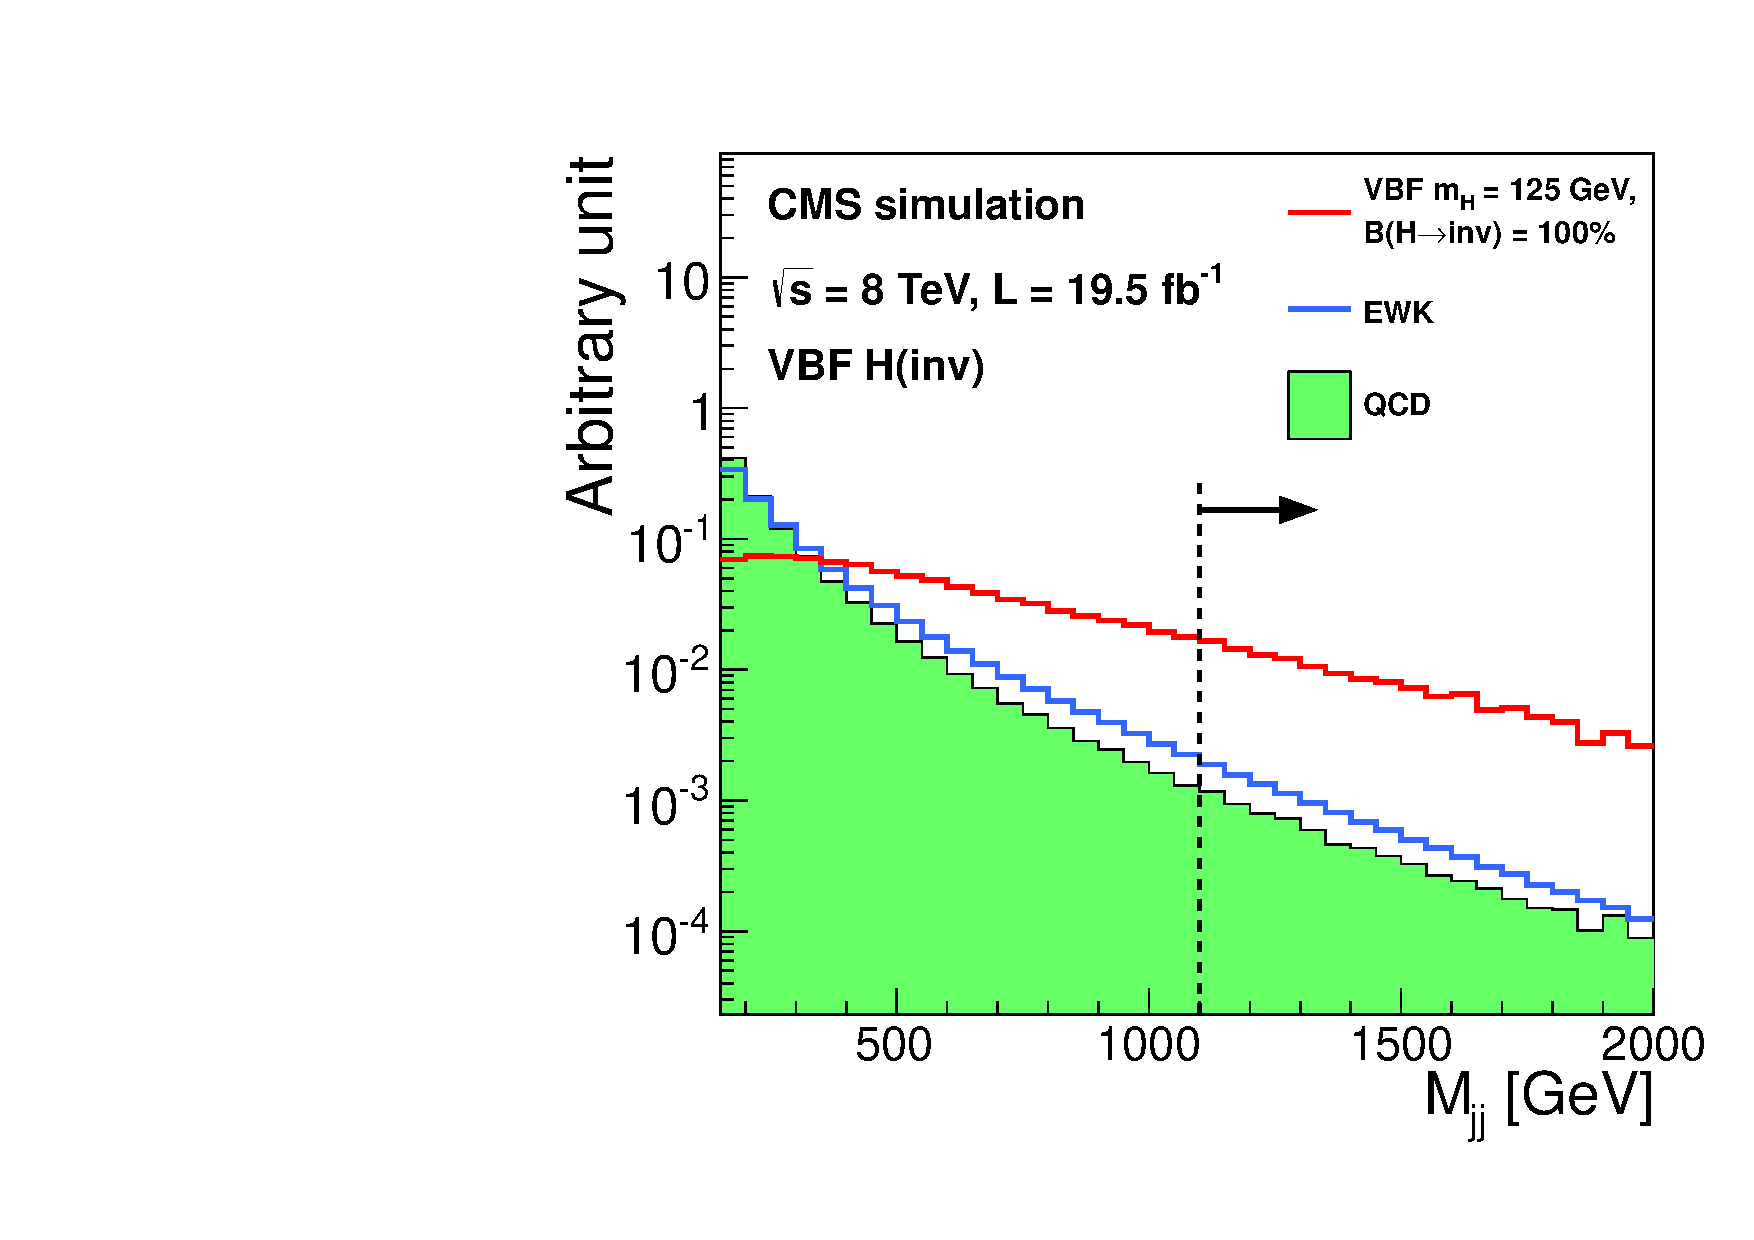
\includegraphics[width=0.45\textwidth]{Chapter05/Images/VBF-Dijet-M.pdf}}\qquad
\subfloat[]{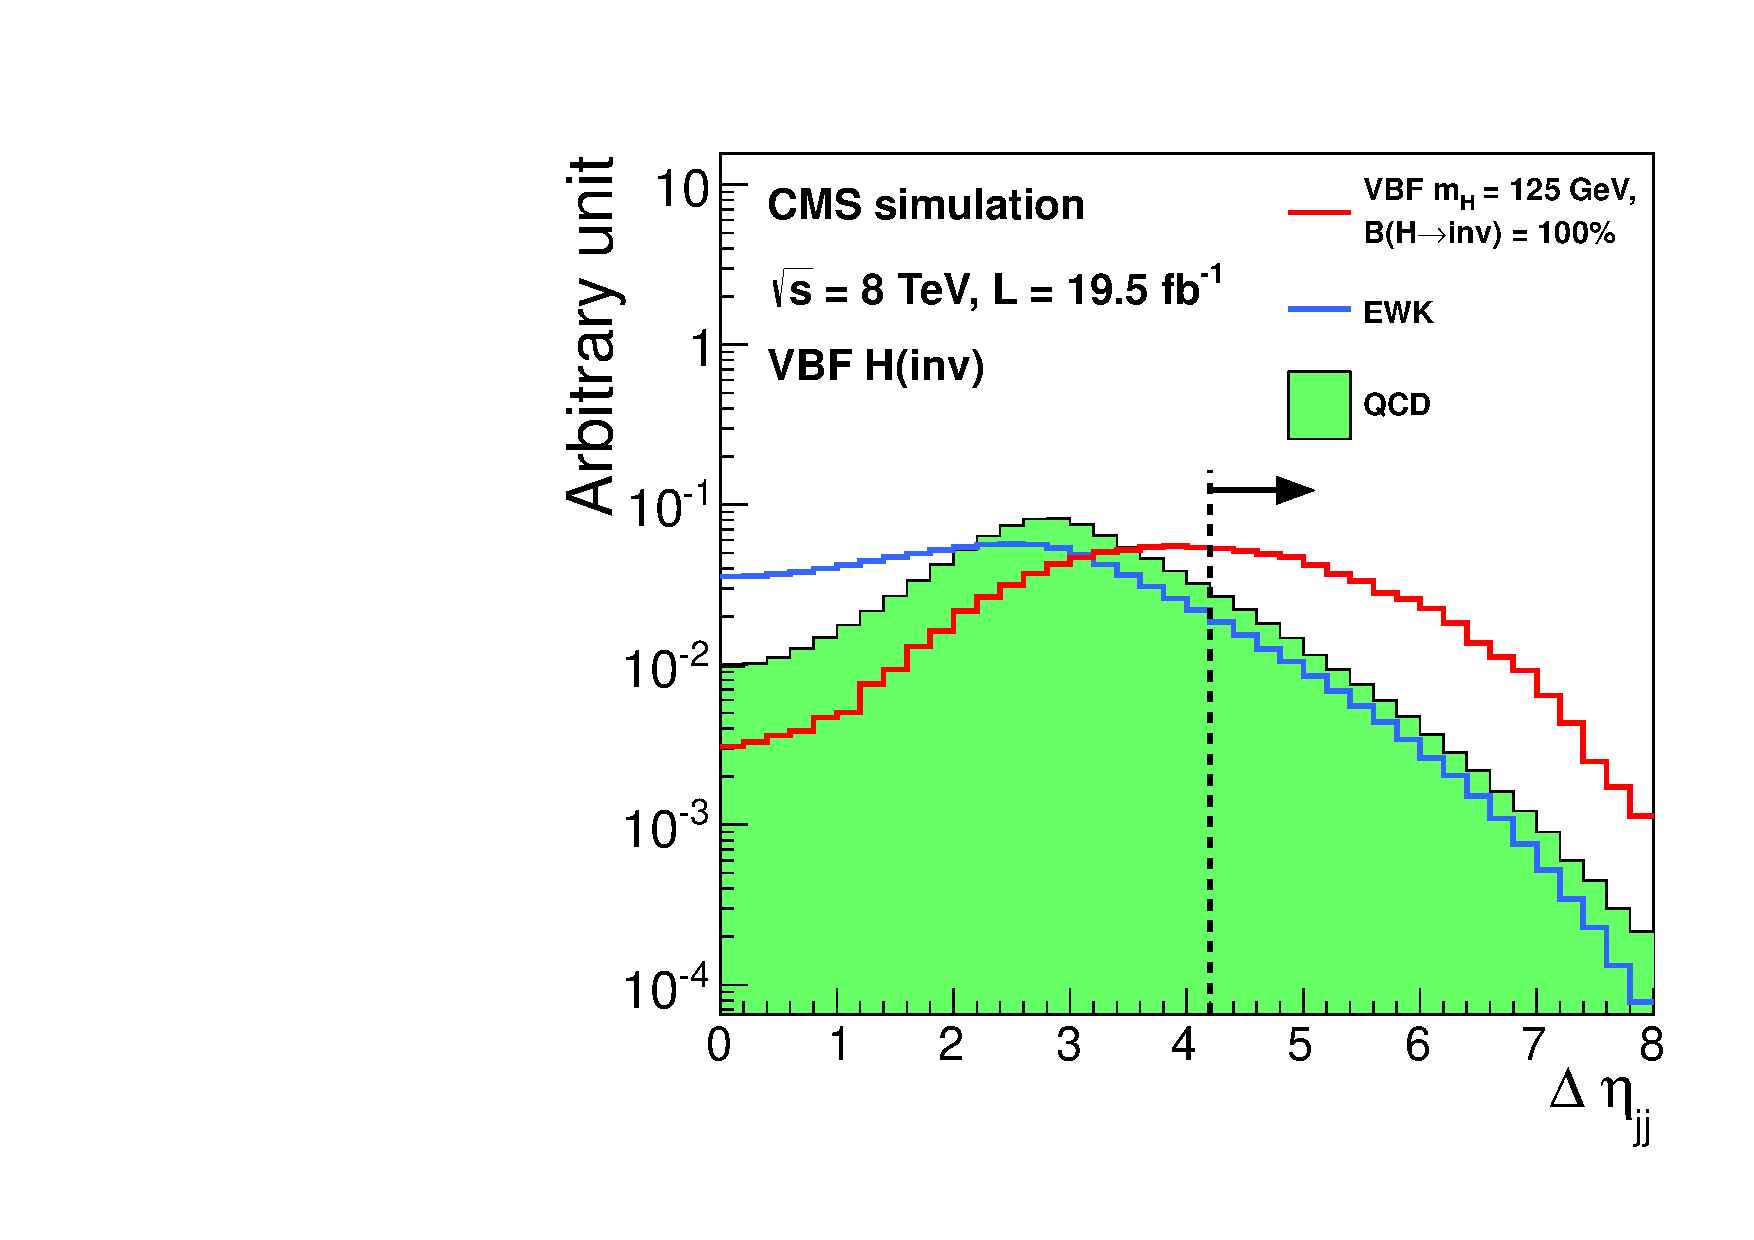
\includegraphics[width=0.45\textwidth]{Chapter05/Images/VBF-Dijet-DEta.pdf}}\\
\subfloat[]{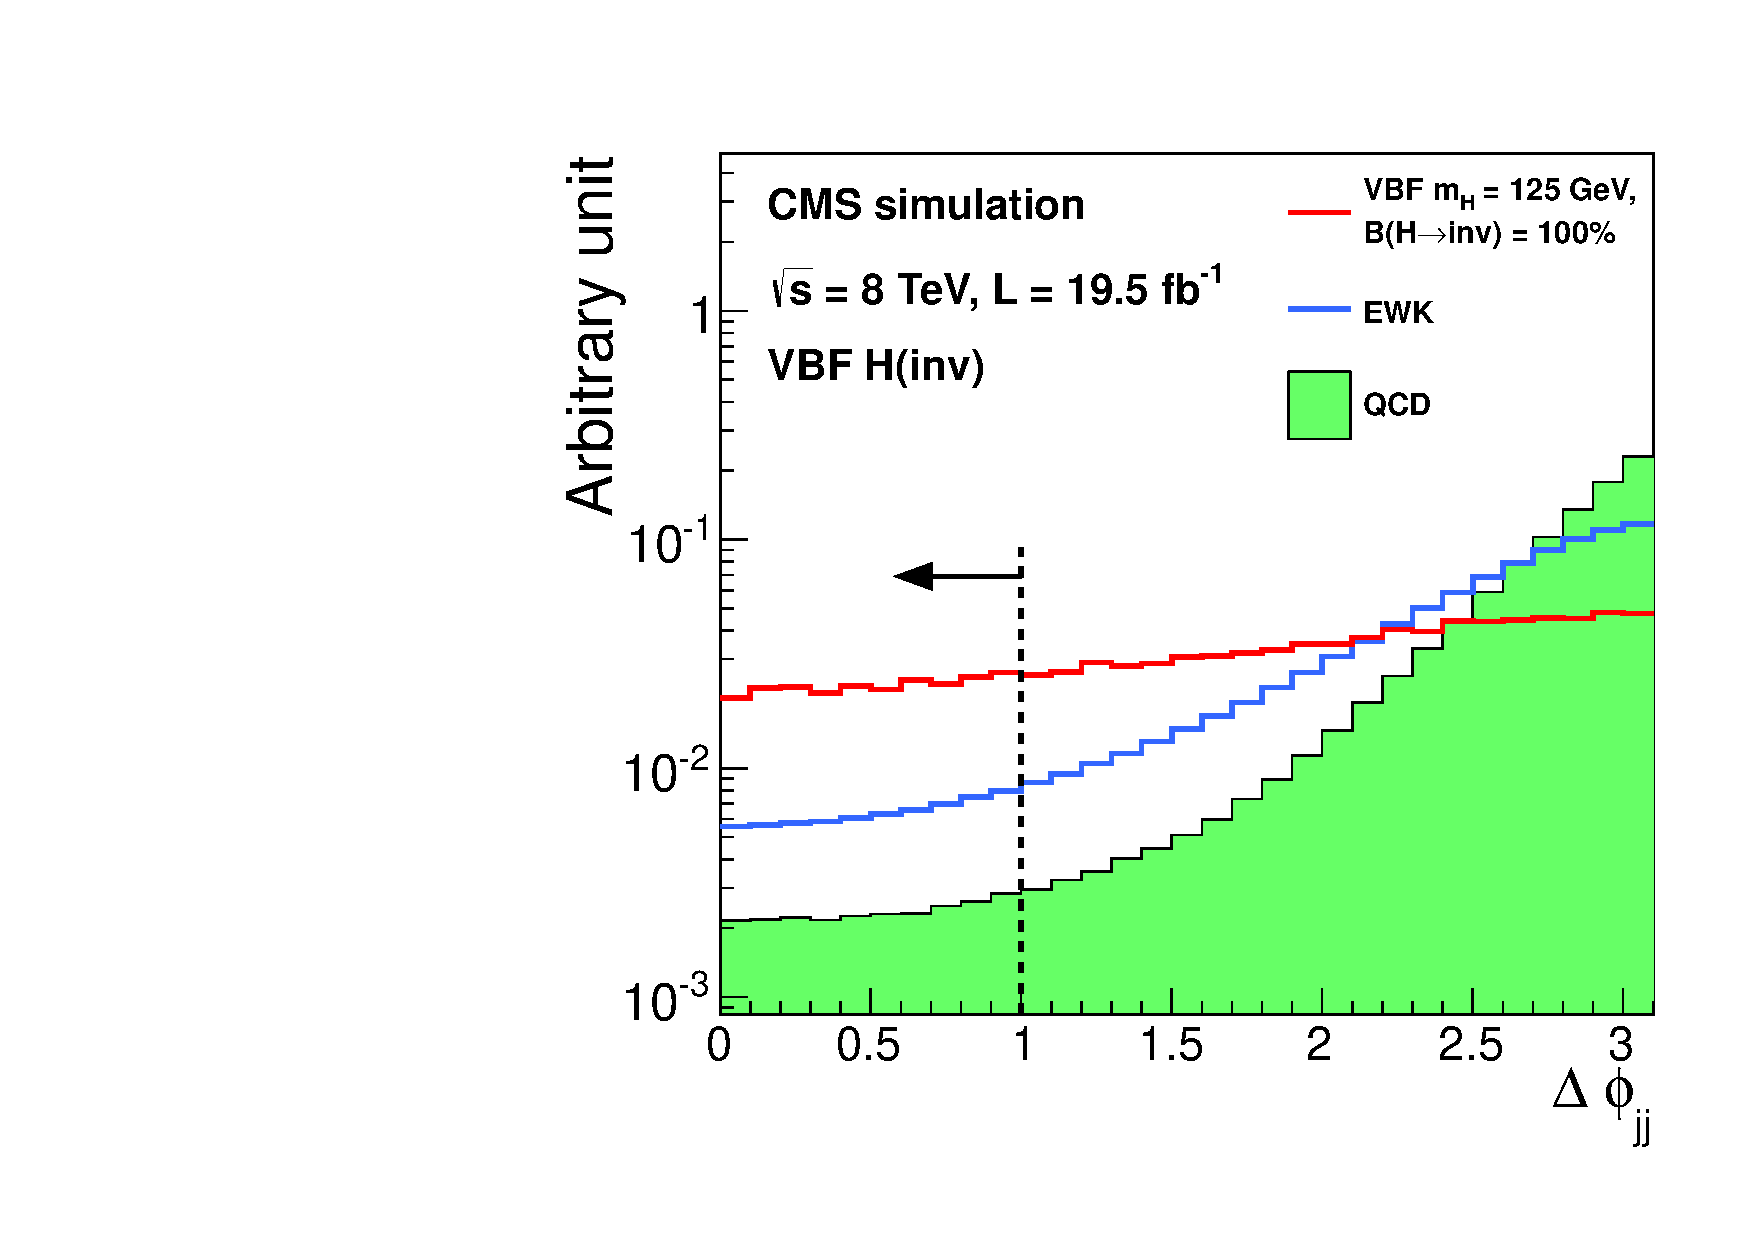
\includegraphics[width=0.45\textwidth]{Chapter05/Images/VBF-Dijet-DPhi.pdf}}\qquad
\subfloat[]{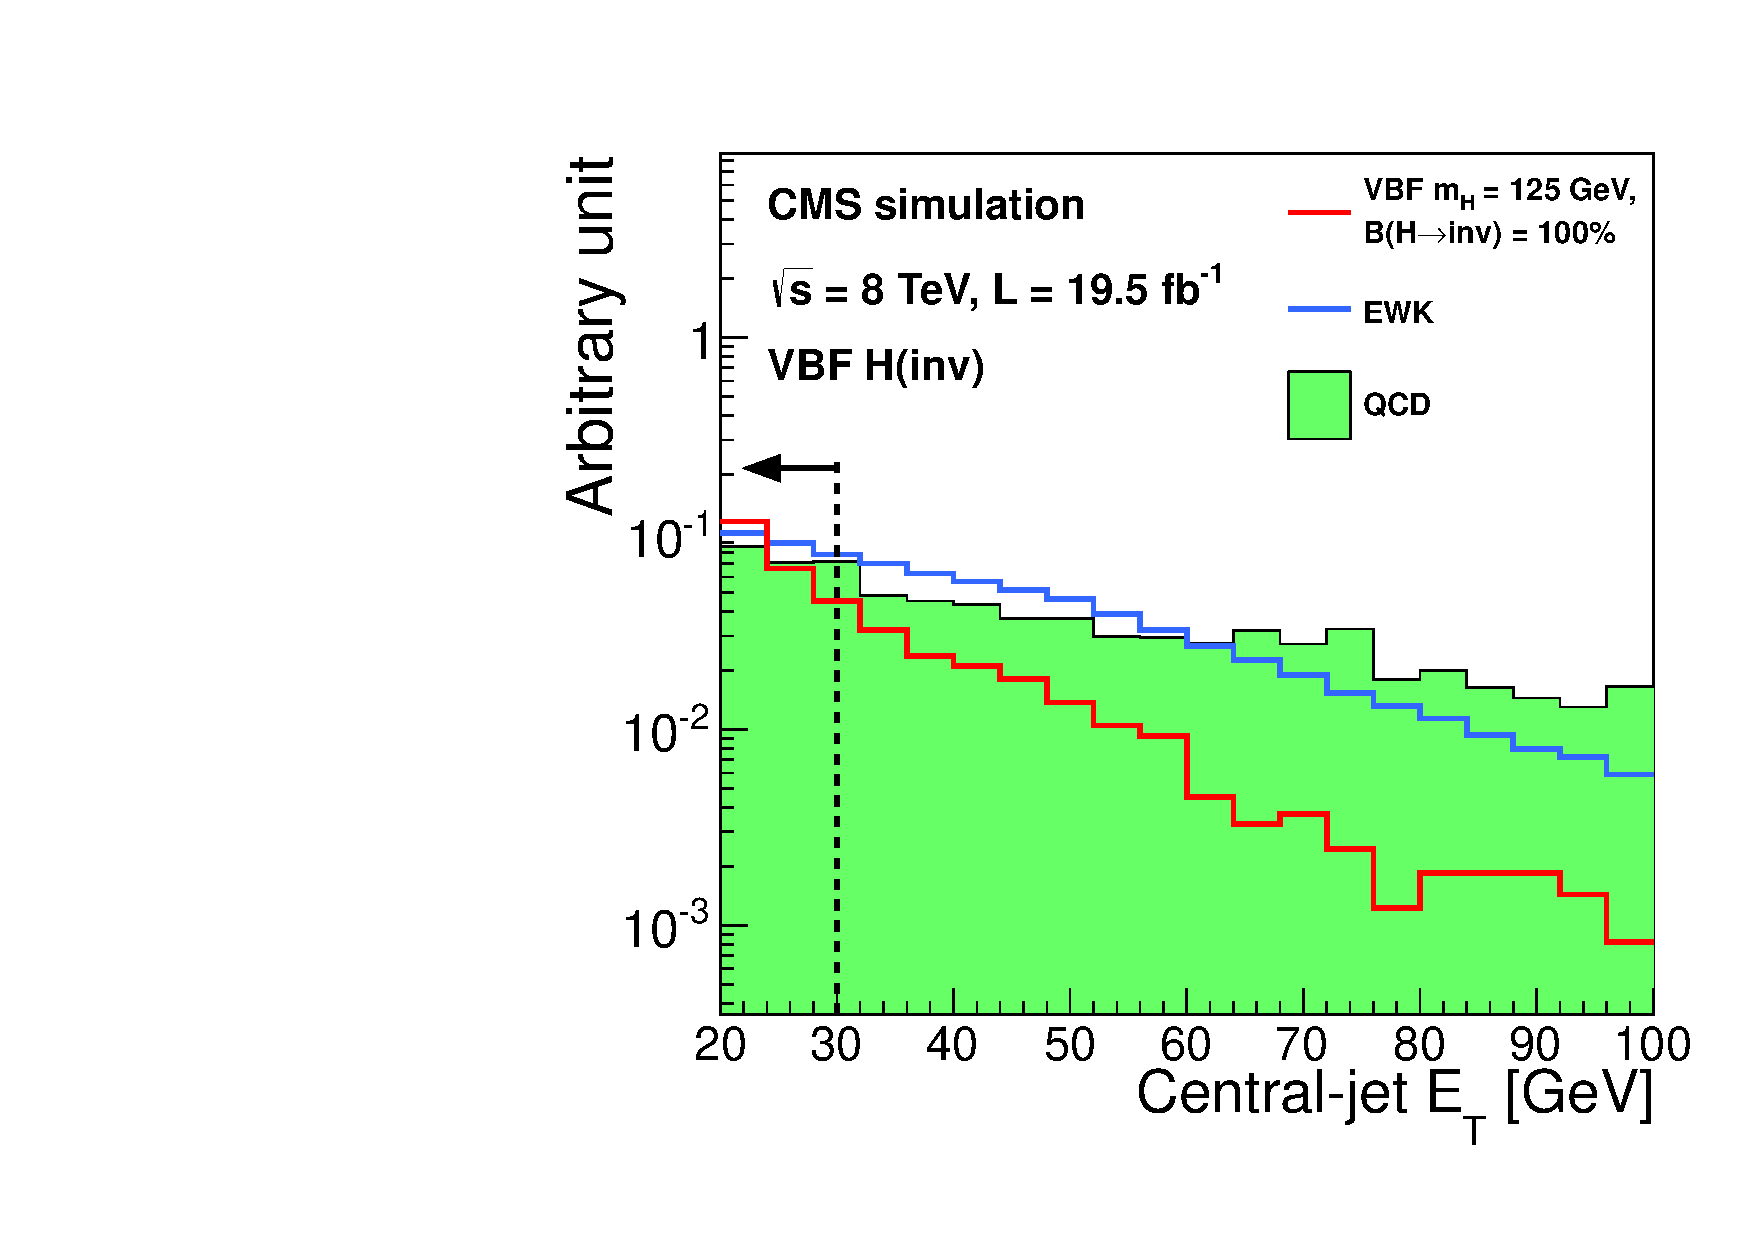
\includegraphics[width=0.45\textwidth]{Chapter05/Images/VBF-CJV-pT.pdf}} 
\caption{Distributions of (a) $M_{jj}$, (b) $\Delta\eta_{jj}$, (c) $\Delta\phi_{jj}$, (d) and central jet \pt in background and signal MC simulation. The distributions are shown after requiring two jets with $\pt^{jet_1},\pt^{jet_2} > 50\,\GeV$, $|\eta| < 4.7$, $\eta_{jet1} \cdot \eta_{jet2} < 0$, $M_{jj}>150\,\GeV$, and $MET > 130\,\GeV$. The arrows correspond to the thresholds applied for the final selection, after optimization. \cite{ARTICLE:CMSVBFHiggsToInvAndZHCombination}}
\label{FIGURE:PromptDataAnalysis_EventSelection_KeyVariables}
\end{figure}

To estimate the signal yields the \textsc{POWHEG} \gls{MC} generator \cite{ARTICLE:POWHEG_2004,ARTICLE:POWHEG_2007,ARTICLE:POWHEG_2009v1,ARTICLE:POWHEG_2009v2,ARTICLE:POWHEG_2010v1,ARTICLE:POWHEG_2010v2,ARTICLE:POWHEG_2011v1,ARTICLE:POWHEG_2011v2} was used to create events with a Higgs boson produced via the \gls{VBF} channel with \gls{SM} couplings and with mass of $125\,\GeV$. The obtained signal efficiency was $(6.8 \pm 0.3) \times 10^{-3}$, which corresponds to an event yield of $210 \pm 29\syst$. The signal efficiency dependency on jet $\pt$, dijet $M_{jj}$, and \gls{MET} are correlated and of comparable amounts. Additionally, a small amount of gluon-fusion signal, where the \gls{ISR} emissions take the role of the \gls{VBF} jets, is also expected to pass the signal event selection. Using the same \gls{MC} event generator this contribution has been estimated to be of $14 \pm 10\syst$ events.

%%%%%%%%%%%%%%%%%%%%%%%%%%%%%%%%%%%%%%%%%%%%%%%%%%%%%%%%%%%%%%%%%%%%%%%%%%%%%%%%%%%%
%%% SECTION
%%%%%%%%%%%%%%%%%%%%%%%%%%%%%%%%%%%%%%%%%%%%%%%%%%%%%%%%%%%%%%%%%%%%%%%%%%%%%%%%%%%%
\section{Background Estimation}
\label{SECTION:PromptDataAnalysis_BackgroundEstimation}

%Status: DONE - (Reviewed x1 J.Pela) (reviewed D. Colling x1)

The irreducible background $\Z(\nu \nu)\text{+jets}$ is estimated from data using as proxy $\Z (\mu \mu)$ decays. A control region for the $\Z$ background is defined with the same event selection as the signal region, with the following changes: instead of the muons veto a pair of opposite charge tight muons is required with an invariant mass compatible with a $\Z$ decay of $60 < M_{\mu\mu}<120\,\GeV$. We veto the event if any more additional veto electrons or loose muons are present. We use $MET_{no-\mu}$ to emulate the signature from a $\Z$ decay into neutrinos. We can extrapolate the number of events in signal region using equation \ref{EQUATION:FIGURE:PromptDataAnalysis_BackgroundEstimation_Zmumu}.

\begin{equation}
N^\mathrm{s}_{\nu\nu} = (N^\mathrm{c}_{\mu\mu\text{obs}} - N^\mathrm{c}_\text{bkg}) \cdot \frac{\sigma(\Z \to \nu\nu)}{\sigma(\Z/\gamma^{*} \to \mu\mu)} \cdot \frac{\varepsilon^\mathrm{s}_{\Z \mathrm{MC}}}{\varepsilon^\mathrm{c}_{\Z \mathrm{MC}}}.
\label{EQUATION:FIGURE:PromptDataAnalysis_BackgroundEstimation_Zmumu}
\end{equation}

%TODO: I think its DY to mumu only. Patrick says yes.

Where $N^\mathrm{s}_{\nu\nu}$ is the estimated number of $\Z(\nu \nu)$ events in the signal region, $N^\mathrm{c}_{\mu\mu\text{obs}}$ is the number of observed events in the control region in data, $N^\mathrm{c}_\text{bkg}$ is the number of other backgrounds events in the control region estimated from simulation, $\sigma(\Z \to \nu \nu) / \sigma(\Z/\gamma^{*} \to \mu \mu)$ is the ratio of cross sections for both $\Z(\nu \nu)$ and $\Z (\mu \mu)$ processes, $\varepsilon^\mathrm{s}_{\Z \mathrm{MC}}$ and  $\varepsilon^\mathrm{c}_{\Z \mathrm{MC}}$ are the $Z$ background selection efficiency for the signal region and control region estimated both from \gls{MC}. The \textsc{MCFM} \gls{MC} generator \cite{ARTICLE:MCFMGenerator} was used to estimate the the ratio of cross sections in equation \ref{EQUATION:FIGURE:PromptDataAnalysis_BackgroundEstimation_Zmumu} as $\sigma(\Z \to \nu \nu) / \sigma(\Z/\gamma^{*} \to \mu \mu) = 5.651 \pm 0.023\syst$ for $m_{\Z/\gamma^{*}} > 50\,\GeV$. The selection efficiency terms are calculated using a DY($\ell\ell$)+jets \gls{MC} simulation, for the signal region the muons are ignored and the obtained efficiency is $\varepsilon^\mathrm{s}_{\Z \mathrm{MC}} = (1.65 \pm 0.27\syst)$ and $\varepsilon^\mathrm{c}_{\Z \mathrm{MC}}=(1.11 \pm 0.17\syst) \times 10^{-6}$ for the control region. The event yield observed in this control region is of $N^\mathrm{c}_{\mu\mu\text{obs}} = 12$ events. The other backgrounds in the control region are estimated using \gls{MC} simulation of the $\ttbar$, diboson and single-top processes being $N^\mathrm{c}_\text{bkg}=0.23 \pm 0.15\syst$ event. Using  these results the contribution of the  $\Z (\nu \nu)$ background in the signal region is estimated as $99 \pm 29\stat \pm 25\syst$ events. Figure \ref{FIGURE:PromptDataAnalysis_BackgroundEstimation_ZControlRegion} shows the \gls{MET} and dijet invariant mass distributions with a less strict $\Z$ control region event selection, where $\Delta\eta_{jj}$, $\Delta\phi_{jj}$ and \gls{CJV} requirements are not enforced and requiring dijet $M_{jj}>1000\,\GeV$. 

\begin{figure}[!htb]
\centering
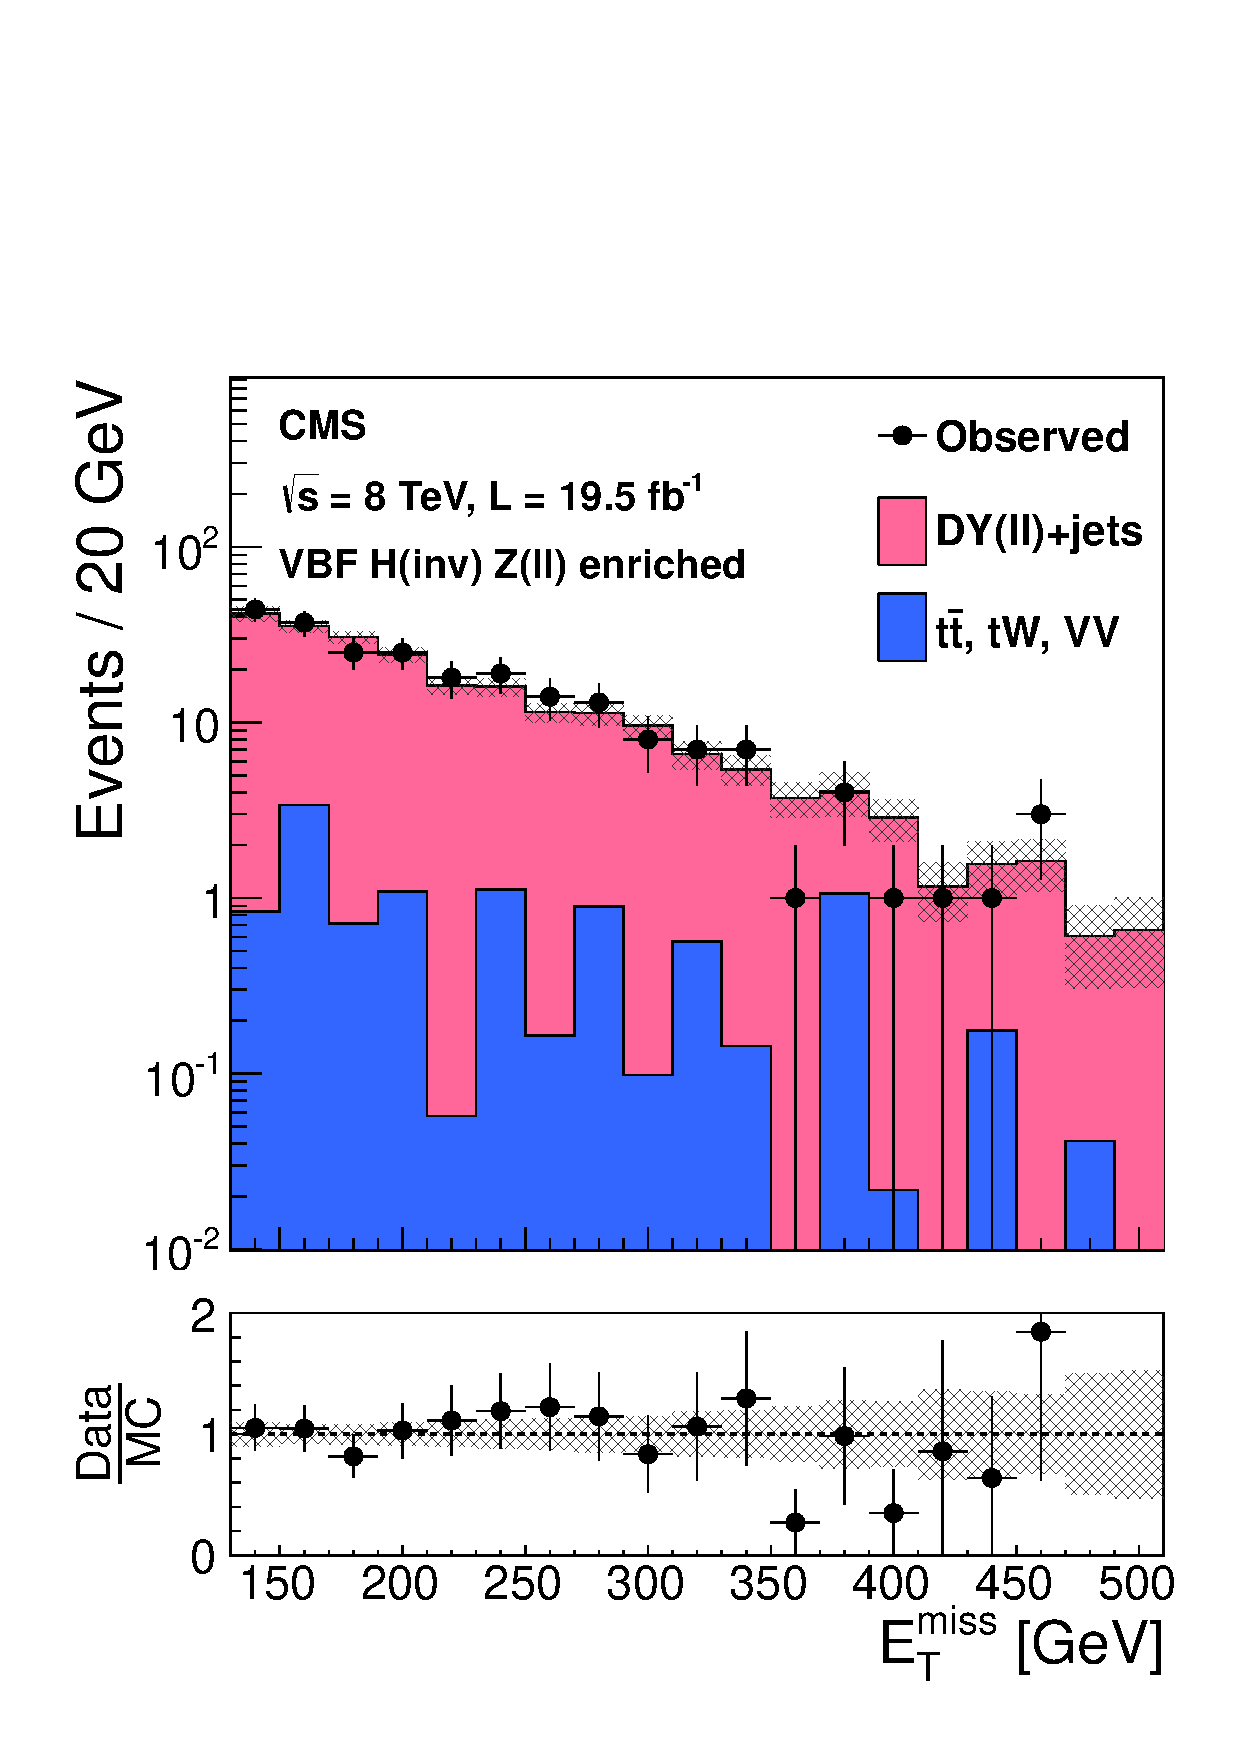
\includegraphics[width=0.45\textwidth]{Chapter05/Images/ZCtrlMET.pdf}
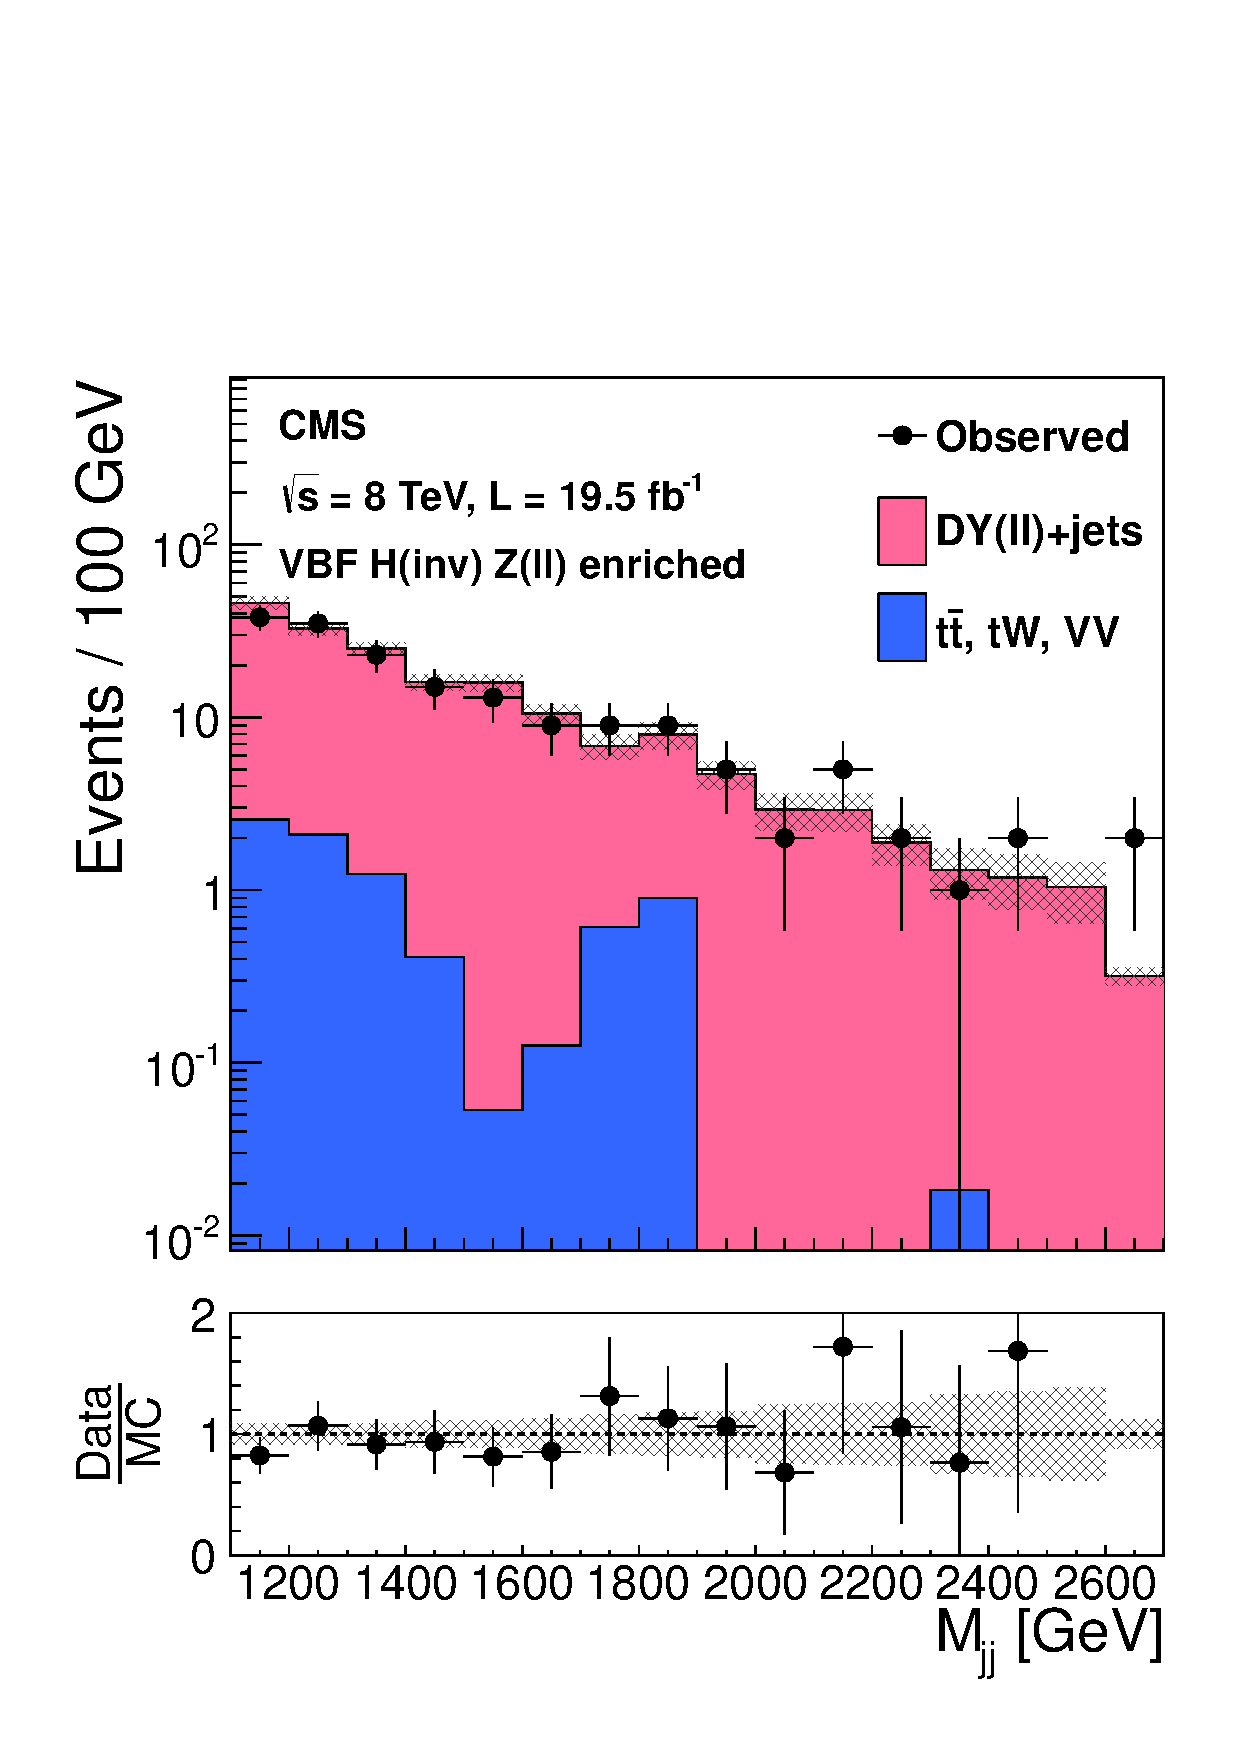
\includegraphics[width=0.45\textwidth]{Chapter05/Images/ZCtrlMjj.pdf}   
\caption{Distribution for \gls{MET} on the right and $M_{jj}$ on the left for a relaxed $Z$ control region, with no requirements on $\Delta\eta_{jj}$, $\Delta\phi_{jj}$, or \gls{CJV} and with a $M_{jj}>1000\,\GeV$ requirement. Backgrounds are shown cumulatively, normalized to data, and with systematic uncertainty shown as a hatched region. The lower panels show the ratio of data to the simulated background. \cite{ARTICLE:CMSVBFHiggsToInvAndZHCombination}}
\label{FIGURE:PromptDataAnalysis_BackgroundEstimation_ZControlRegion}
\end{figure}

The $\W$ boson backgrounds, $\PW (\Pe \nu)\text{+jets}$ and $\PW (\mu \nu)\text{+jets}$, are estimated in control regions that select a single lepton. Two regions are defined following the approach used for the $\Z$ boson background. The $\PW (\mu \nu)$ control region is defined by replacing the \textit{loose muon} veto by a requirement of one \textit{tight muon} and vetoing any event with additional \textit{loose muons}. For this control region the $MET_{no-\mu}$ is used to replicate what would be expected if the muon was miss reconstructed or miss identified. The $\PW (\Pe \nu)$ control region is defined by replacing the electron veto by a requirement of one \textit{tight electron} and vetoing any event with additional \textit{veto electrons}. For this control region we do not recompute \gls{MET} as it is included in the trigger requirements. Equation \ref{EQUATION:PromptDataAnalysis_BackgroundEstimation_WLep} can be used to extrapolate the events in both this control regions to the signal region.

\begin{equation}
N^\mathrm{s}_\ell = (N^\mathrm{c}_{\ell\text{obs}} - N^\mathrm{c}_\text{bkg}) \cdot \frac{N^\mathrm{s}_{\PW \mathrm{MC}}}{N^\mathrm{c}_{\PW \mathrm{MC}}},
\label{EQUATION:PromptDataAnalysis_BackgroundEstimation_WLep}
\end{equation}

Where $N^\mathrm{s}_\ell$ is the estimated number of background events in the signal region, $N^\mathrm{c}_{\ell\text{obs}}$ is the number of observed events in the control region in data, $N^\mathrm{c}_\text{bkg}$ is the number of other backgrounds in the control region estimated from simulation, $N^\mathrm{s}_{\PW \mathrm{MC}}$ and $N^\mathrm{c}_{\PW \mathrm{MC}}$  are the number of $\PW (\ell \nu)\text{+jets}$ background events in signal and control regions estimated from \gls{MC} simulation. These ratios are estimated and $N^\mathrm{s}_{\PW \mathrm{MC}}/N^\mathrm{c}_{\PW \mathrm{MC}}$ is equal to $0.347 \pm 0.045\syst$ for $\PW (\mu \nu)$ and $1.08 \pm 0.21\syst$ for $\PW (\Pe \nu)$. In data the observed yields is the $\PW (\mu \nu)$ control region is 223 events, with estimated backgrounds from other processes of $30.4 \pm 7.0\syst$ events. For the $\PW (\Pe \nu)$ control region the observed yield is 65 events with estimated backgrounds from other processes of $7.1 \pm 4.7\syst$ events. The  extrapolated background in the signal region is $66.8 \pm 5.2\stat \pm 15.7\syst$ events for the $\PW (\mu \nu)$ background and  $62.7 \pm 8.7\stat \pm 18.1\syst$ for the $\PW (\Pe \nu)$ background.

The $\PW (\tau \nu)\text{+jets}$ process where the tau decays hadronically $\tau_{had}$ is estimated in a similar way to $\PW (\Pe \nu)\text{+jets}$ and $\PW (\mu \nu)\text{+jets}$. The $\PW (\tau_{had} \nu)$ control region is defined like the signal region with the additional requirement of one tau following the description of chapter \ref{CHAPTER:EventReconstructionAndSimulation}, no other additional lepton are allowed, and the \gls{CJV} is not applied to increase the yield. We estimated the yield in the signal region $N^\mathrm{s}_{\tau_{had}}$ using equation \ref{EQUATION:PromptDataAnalysis_BackgroundEstimation_WLep}. The conversion factor is derived again from the prediction of the number of events in the signal and control regions for this process from \gls{MC} simulation. The extrapolated signal region contribution for the $\PW (\tau_{had} \nu)$ background of $53 \pm 18\stat \pm 18\syst$ events.

To increase the confidence in the \gls{MC} background model and the extrapolations to the signal regions, we compute the expected data yields from one control regions to another using conversion factors determined from \gls{MC} simulation. For example, the $\PW (\mu \nu)$ control region data yield is used to compute the yield of the the $\Z (\mu \mu)$ region as given by using equation \ref{EQUATION:PromptDataAnalysis_BackgroundEstimation_RegionCrossCheck}. In all cases, the estimations agreed, within uncertainties, with the observed yields in data. 

\begin{equation}
N^\mathrm{c}_{\mu \mu} = (N^\mathrm{c}_{\mu \text{obs}} - N^\mathrm{c}_\text{bkg}) \cdot \frac{N^\mathrm{c}_{\Z \mathrm{MC}}}{N^\mathrm{c}_{\PW \mathrm{MC}}},
\label{EQUATION:PromptDataAnalysis_BackgroundEstimation_RegionCrossCheck}
\end{equation}

The \gls{QCD} multijet background is estimated in the signal region by defining four regions depending or passing or failing the \gls{MET} and \gls{CJV} requirements. We define these regions after the full remaining selection as follows:

\begin{itemize}
  \item{A: fail \gls{MET} criteria, fail \gls{CJV} criteria;}
  \item{B: pass \gls{MET} criteria, fail \gls{CJV} criteria;}
  \item{C: fail \gls{MET} criteria, pass \gls{CJV} criteria;}
  \item{D: pass \gls{MET} criteria, pass \gls{CJV} criteria.}
\end{itemize}

We use regions A, B and C to estimate the \gls{QCD} multijet contribution in D. These three regions are first subtracted of the electroweak backgrounds, which are already estimated using other control regions, with event yield estimations from \gls{MC} simulation. The \gls{QCD} multijet yield in region D is then estimated using $N_\mathrm{D} = N_\mathrm{B}N_\mathrm{C} / N_\mathrm{A}$ where $N_{i}$ is the number of events in region $i$. This method is based on the assumption that the four regions are uncorrelated, which is tested by comparing the \gls{MET} distributions below $MET < 130\,\GeV$ of both pass and fail \gls{CJV}. The maximum observed difference was of 40\%, which is assigned as a method systematic. Using this method the contribution to signal region of \gls{QCD} multijets processes is of $30.9 \pm 4.8\stat \pm 23.0\syst$. To increase the confidence on this method, it was applied to a \gls{QCD} multijet dominated area by changing the $\Delta\phi_{jj}$ requirement to $\Delta\phi_{jj}>2.6\,\radian$. In this region $2551 \pm 57\stat$ events were observed, after subtraction of other backgrounds which were estimated from \gls{MC} simulation. The prediction of this method is of $2959 \pm 58\stat$ events, which is compatible with the observation within systematic uncertainties. Furthermore, a cross-check was performed using as variables \gls{MET} and $\Delta\phi_{jj}$, the obtained predictions is consistent with the main method.

The remaining \gls{SM} background, for the processes $\ttbar$, single-top, VV and DY($\ell\ell$)+jets, in the signal region are estimated  directly form \gls{MC} simulation to be $20.0 ^{+6.0}_{-8.2}\syst$ events. Table \ref{TABLE:PromptDataAnalysis_BackgroundEstimation_BackgroundSummary} summarizes all background estimations along with the prediction of the yield for a signal with $m_{H}=125\,\GeV$ and $\BRinv=100$\%. The total expected background yield in the signal region is $332 \pm 36\stat \pm 45\syst$. 

\begin{table}[!htb]
\centering
\begin{tabular}{|l|c|}
\hline
Process                                  & Event yields                  \\
\hline\hline
$\Z (\nu\nu)\text{+jets}$                & $  99 \pm  29 \stat \pm 25 \syst$  \\
$\PW (\mu\nu)\text{+jets}$               & $  67 \pm   5 \stat \pm 16 \syst$   \\
$\PW (\Pe \nu)\text{+jets}$              & $  63 \pm   9 \stat \pm 18 \syst$   \\
$\PW (\tau_{had} \nu)\text{+jets}$       & $  53 \pm  18 \stat \pm 18 \syst$  \\
QCD multijet                             & $  31 \pm   5 \stat \pm 23 \syst$   \\
Sum (\ttbar, single top quark, $VV$, DY) & $20.0 \pm 8.2 \syst$ \\
\hline\hline
Total background                         & $332 \pm 36 \stat \pm 45 \syst$ \\
VBF H(inv.)                              & $210 \pm 29 \syst$ \\
ggF H(inv.)                              & $ 14 \pm 10 \syst$ \\
Observed data                            & 390  \\
\hline\hline
S/B                                      & 70\% \\
\hline
\end{tabular}
\caption{Summary of the estimated number of background and signal events, together with the observed yield, in the \gls{VBF} search signal region. The signal yield is given for $m_H=125\,\GeV$ and $\BRinv=100$\%. \cite{ARTICLE:CMSVBFHiggsToInvAndZHCombination}}
\label{TABLE:PromptDataAnalysis_BackgroundEstimation_BackgroundSummary}
\end{table}

%%%%%%%%%%%%%%%%%%%%%%%%%%%%%%%%%%%%%%%%%%%%%%%%%%%%%%%%%%%%%%%%%%%%%%%%%%%%%%%%%%%%
%%% SECTION
%%%%%%%%%%%%%%%%%%%%%%%%%%%%%%%%%%%%%%%%%%%%%%%%%%%%%%%%%%%%%%%%%%%%%%%%%%%%%%%%%%%%
\section{Sources of uncertainty}
\label{SECTION:PromptDataAnalysis_SourcesOfUncertainty}

%Status: DONE - (Reviewed x1 J.Pela) (reviewed D. Colling x1)

The data control event samples for V+jets backgrounds small size translates into a large statistical uncertainty on the estimates in the signal region ranging from $5-30\%$. The systematic uncertainty also associated with this channels is dominated by the \gls{MC} samples statistical uncertainty when calculating the conversion factors from control to signal regions. Important sources of systematic uncertainty also arise from the effects of the jet and \gls{MET} energy scale and resolution. These effects are estimate by varying the scales and resolutions within their uncertainty, applying them to the jets and unclustered energy and recalculating the \gls{MET}. Resulting in a systematic uncertainty of 13\% in the signal acceptance, 7-15\% in the V+jets background estimates, and 60\% uncertainty in the \gls{QCD} multijet background estimate. As described in the previous section an additional uncertainty of 40\% is associated with the \gls{QCD} multijet estimation, but this background yield is small compared with the total. Muon and electron efficiency uncertainties appear due to the scale factors used to correct \gls{MC} simulation to data and are small. 

For the minor backgrounds which were estimated from \gls{MC} simulation, the dominating uncertainties come from the used physics process cross sections, which are set according to measurements made by other \gls{CMS} collaboration analyses, and the jet/\gls{MET} scale uncertainties. Theoretical uncertainties on the \gls{VBF} signal yields result from \gls{PDF} uncertainties, factorization and renormalization scale uncertainties. For the gluon fusion signal the dominating uncertainties arise from \gls{MC} modelling of \gls{ISR} and other effects. It is estimated by comparing the estimates from different \gls{MC} generators and is estimated to be 60\%. Gluon fusion represents a small amount of the total signal so this uncertainty only has a modest effect. Table \ref{TABLE:PromptDataAnalysis_SourcesUncertaintySummary} summarizes the uncertainties taken into account in relation to signal or total background yields. The combined effect of all uncertainties associated with the backgrounds results in an increase of about 65\% in the expected upper limit on the \BRinv.

\begin{table}[!htb]
\centering
\begin{tabular}{|l|c|c|}
\hline
Source                                           & Total background & Signal \\
\hline\hline
Control region statistics                        & 11\%             & -      \\
MC statistics                                    & 11\%             & 4\%    \\
Jet/$E_T^{\text{miss}}$ energy scale/resolution  & 7\%              & 13\%   \\
QCD background estimation                        & 4\%              & -      \\
Lepton efficiency                                & 2\%              & -      \\
Tau ID efficiency                                & 1\%              & -      \\
Luminosity                                       & 0.2\%            & 2.6\%  \\
Cross sections                                   & 0.5--1\%         & -      \\
PDFs                                             & -                & 5\%    \\
Factorization/renormalization scale              & -                & 4\%    \\
Gluon fusion signal modelling                    & -                & 4\%    \\
\hline\hline
Total                                            & 18\%             & 14\%   \\
\hline 
\end{tabular}
\caption{Summary of the uncertainties in the total background and signal yields in the \gls{VBF} channel. All uncertainties affect the normalization of the yield, and are quoted as the change in the total background or signal estimate, when each systematic effect is varied according to its uncertainties. The signal uncertainties are given for $m_H=125\,\GeV$ and $\BRinv=100$\%. \cite{ARTICLE:CMSVBFHiggsToInvAndZHCombination}}
\label{TABLE:PromptDataAnalysis_SourcesUncertaintySummary}
\end{table}


%%%%%%%%%%%%%%%%%%%%%%%%%%%%%%%%%%%%%%%%%%%%%%%%%%%%%%%%%%%%%%%%%%%%%%%%%%%%%%%%%%%%
%%% SECTION
%%%%%%%%%%%%%%%%%%%%%%%%%%%%%%%%%%%%%%%%%%%%%%%%%%%%%%%%%%%%%%%%%%%%%%%%%%%%%%%%%%%%
\section{Results and conclusions}

%Status: DONE - (Reviewed x1 J.Pela) (reviewed D. Colling x1)

As shown in table \ref{TABLE:PromptDataAnalysis_BackgroundEstimation_BackgroundSummary}, 390 data events were observed in the signal region, this yield is compatible with the background only prediction. Since no evidence of signal is observed 95\% \gls{CL} upper limits on the Higgs boson production cross section times branching fraction are computed. The limits are calculated using the $\mathrm{CL}_\mathrm{s}$ method \cite{ARTICLE:HandbookofLHCHiggsCrossSectionsDifferentialDistributions,ARTICLE:CLsTechnique,ARTICLE:CLCompForCombiningSearchesWithSmallStat} based on asymptotic formulae \cite{ARTICLE:AsymptoticCLS}, following the standard \gls{CMS} Higgs boson searches combination technique \cite{ARTICLE:CMS_HiggsDiscovery,ARTICLE:HiggsCombination}. Systematic uncertainties are incorporated as nuisance parameters and treated according to the frequentist paradigm \cite{ARTICLE:HiggsCombination}. The 95\% \gls{CL} limits on the Higgs boson production cross section times invisible branching fraction are also presented normalised to the \gls{SM} production cross section \cite{ARTICLE:HandbookofLHCHiggsCrossSectionsInclusiveObservables,ARTICLE:HandbookofLHCHiggsCrossSectionsDifferentialDistributions}, which is denoted as $\xi = \sigma \cdot \BRinv / \sigma_\mathrm{SM}$. The choice of the \gls{SM} production cross section is arbitrary, since in the existence of a sizeable invisible cross section width would indicate physics beyond the \gls{SM}, which could mean also modification of the production cross-sections. An alternative choice of model for Higgs boson production would not provide additional information since it essentially would scale the limits.

If \gls{SM} production cross sections and acceptances are assumed, $\xi$ can be interpreted as a limit on the invisible branching the  of the $125\,\GeV$ Higgs boson.

Figure \ref{FIGURE:PromptDataAnalysis_VBFLimit} shows on the left plot the observed and median expected 95\% \gls{CL} limits on the Higgs boson production cross section times invisible branching fraction, as a function of the Higgs boson mass, for the \gls{VBF} production mode. The right plot shows the corresponding limit on $\xi$.  Assuming the \gls{SM} \gls{VBF} production cross section and acceptance, this corresponds to an observed (expected) upper limit on \BRinv of 0.65 (0.49) for $m_H=125\,\GeV$.

\begin{figure}[!htp]
\centering
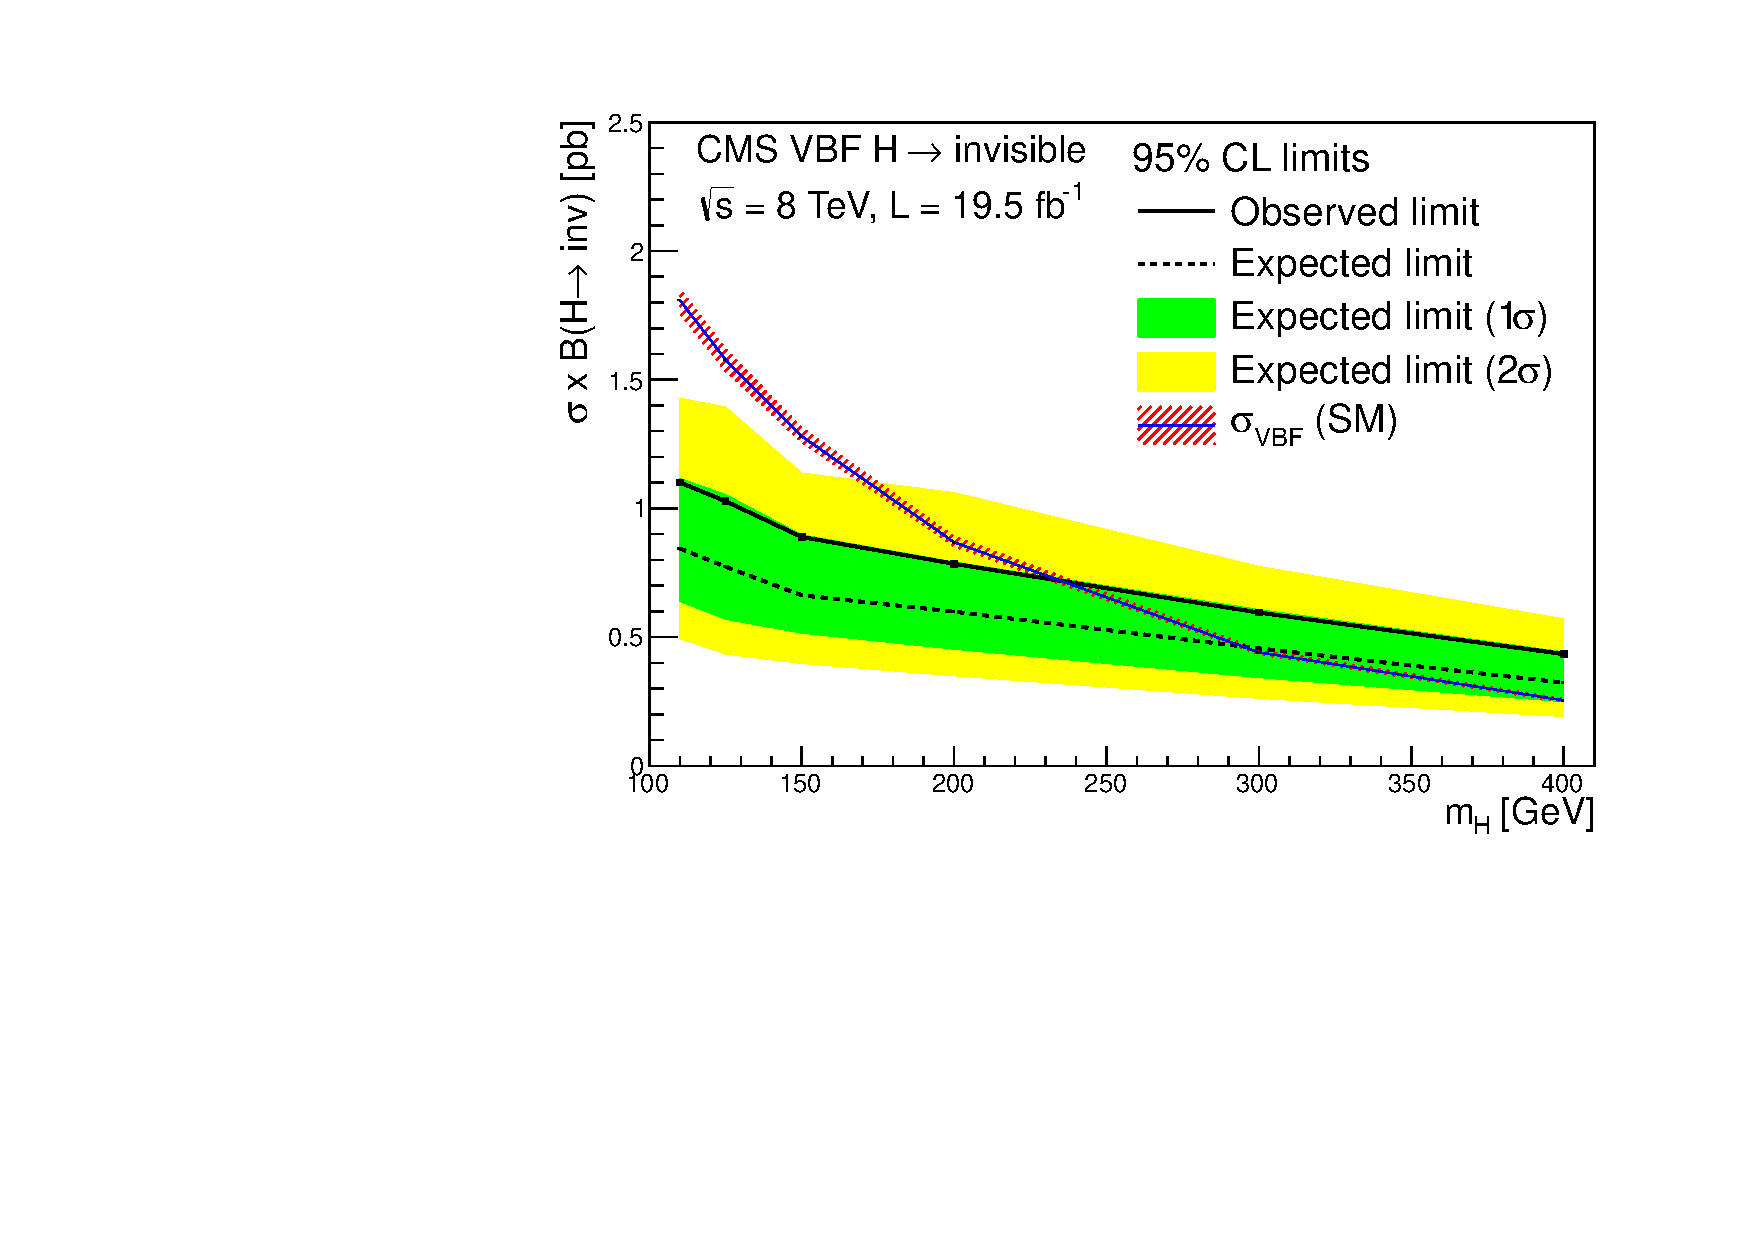
\includegraphics[width=0.49\textwidth]{Chapter05/Images/vbfxslimit.pdf}
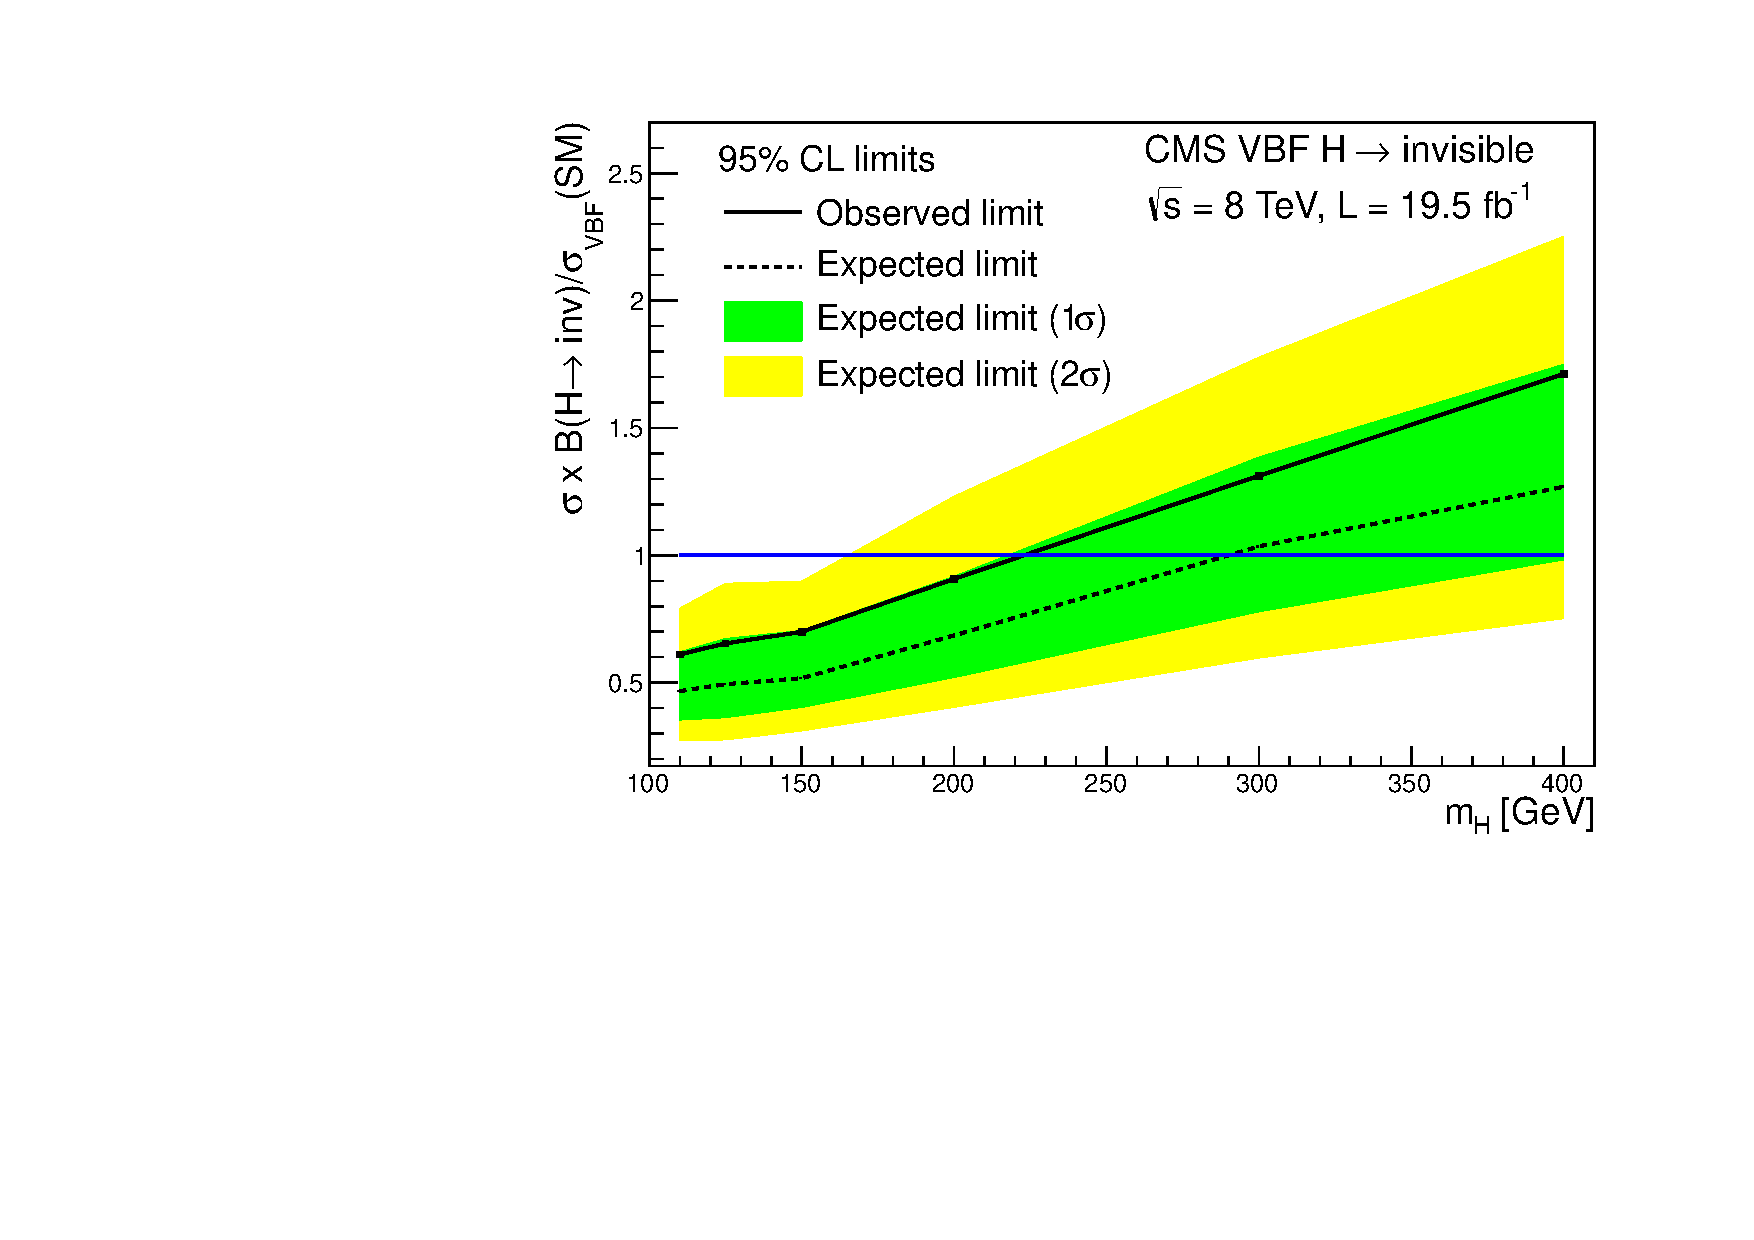
\includegraphics[width=0.49\textwidth]{Chapter05/Images/vbflimit.pdf}
\caption{Expected and observed 95\% CL upper limits on the VBF production cross section times invisible branching fraction (left figure), and normalized to the \gls{SM} Higgs boson \gls{VBF} production cross section (right figure). \cite{ARTICLE:CMSVBFHiggsToInvAndZHCombination}}
\label{FIGURE:PromptDataAnalysis_VBFLimit}
\end{figure}
